\documentclass[runningheads,a4paper]{llncs}
%\documentclass[a4paper,11pt]{report}
\usepackage{color,graphicx,url,wrapfig,glossaries,appendix,epigraph}
\graphicspath{{./images/}}
%\usepackage[dvips, bookmarks=true, unicode=true, breaklinks=true, pdftitle={Environment execution service}, pdfauthor={Aram Verstegen}, pdfsubject={Technical Computer Science - Bachelor's thesis}, pdfkeywords={NFC, mobile phones}]{hyperref}
%\makenomenclature
\makeglossaries
\begin{document}
\newcommand{\mytitle}{Security of NFC-enabled mobile devices}
\newcommand{\myauthor}{Aram Verstegen \& Mark Vijfvinkel}
\newcommand{\mycourse}{Research \& Development - Research 1, 2010-2011}
\pagenumbering{Roman}
\author{\myauthor}
\title{\mytitle}
\institute{Radboud Universiteit Nijmegen \\ \mycourse}
\maketitle

\begin{flushleft}
\emph{Date:} \hfill \today \\
\emph{Title:} \hfill  \mytitle \\
\emph{Authors:} \hfill \myauthor \\
\emph{Course:} \hfill \mycourse \\
%\emph{Problem:} \hfill \\
\end{flushleft}

\begin{abstract}
New developments in mobile networking technology, which are intended to be used for payment and access control, deserve the attention of security researchers.
This paper aims to serve as both a general and a security-related introduction to mobile-phone based Near Field Communication systems.
\end{abstract}



%\newpage

%\tableofcontents
%\newpage

%\listoffigures
%\listoftables
%\printnomenclature
%\cleardoublepage

\setcounter{page}{1}
\pagenumbering{arabic}

\section{Introduction}
%\newglossaryentry{PKI}{name={Public Key Infrastructure},description={A cryptographic methode for encrypting messages over untrusted networks.}}
%\glsadd{PKI}

%\section*{Purpose}

\subsection{Near Field Communication} %(beetje dubbel)
Near Field Communication (NFC) is an upcoming wireless communication technology which will allow for new applications on mobile devices, e.g. smartphones.
It is an extension of the RFID protocol which allows these devices to assume the capabilities of an RFID card or reader, or utilize an RFID connection interactively.
 
NFC will allow a mobile device to communicate wirelessly over a short distance with other NFC-capable devices such as another smartphone, a payment terminal, a so-called 'smart poster' or an access control terminal.
While \textit{Wireless Personal Area Network} (WPAN) technlogy for mobile devices is already widely deployed in the form of Bluetooth, NFC adds security features also relied upon by RFID which cause it to be considered applicable for security use cases.

%There are two major use cases that sparked its development, namely mobile payments and access control. %MARK we zouden access control toch niet meer gebruiken?

%For users of a mobile device NFC will increase the ease of use, because the user will be able to use a mobile device for paying (e.g. at a shop or candy machine) and use the same device to pay for public transport.
%Theoretically the user doesn't have to carry a wallet anymore, only the mobile device.
%For example, instead of using coins to pay for candy, you'll just wave your smartphone in front of the machine, you'll pay for the candy and the money will be taken out of your bank account. 

%plaatje van een NFC betaling

%TODO Telco's en gebruikers er bij
%TODO Manufacturers of what? - telefoons, NFC tags, ???
%\section{Stakeholders} % was dit niet overbodig om te noemen? MARK: volgens mij zei erik of alles noemen of eruit?
%NFC will be exploited by different stakeholders of the NFC Forum, which was started in 2004 to advance NFC technology.
%Stakeholders are hardware component manufacturers, mobile device assembling companies, SIM card producers, application developers and financial service institutions.
%And of course, let's not forget the user.
%Currently the Forum has 140 members, who all work together to promote the use of NFC. 
%Recently a few pilots have started in the Netherlands which allow users to pay with their mobile device and gain access.
%(misschien hier het voorbeeld noemen van OV chipkaart op de telefoon van Erik Poll).

%\subsection{Implementation}
This allows for new applications to be built on top of existing RFID technology, of which payment and public transport applications are the most important.
RFID-based applications for access control and public transport payment are already in place, and are likely to make the transition to NFC-enabled mobile phones.

\subsection{Motivation}
In our opinion, this trend warrants some serious security research. To our delight, there is already a wealth of literature available on the subject.

However, to our knowledge there has been no succinct, definitive overview leading from the system organisation to the security architecture and the known vulnerabilities of NFC systems.
% "Did you google scholar around for this?"
What we hope to accomplish with this paper is to provide the reader with an introduction to NFC security-related research currently ongoing.
%In addition to this we hope to be able to identify specific applications in which we foresee vulnerabilities.
% "Introduction to NFC security _research_"
% vs "Introduction to NFC security _issues/architecture_"
% Naar welk aspect kijken wij? - Verderop in 1.5 geven jullie hier beter antwoord op


%\subsection{Overview}
%%In chapter \ref{chap:applications} we will briefly summarize some of the applications NFC will likely be used for.
%In chapter \ref{chap:hardware_architecture} we will present an overview of the hardware, software and communication architecture of a NFC-enabled mobile device.
%%\section{...}
%%Further we will look into the possibilities that NFC offers.
%In chapter \ref{chap:known_vulnerabilities} we will summarize security issues on vulnerabilities in NFC or NFC-like applications.

%Based on the architecture and these vulnerabilities, we present a number of foreseen vulnerabilities and explain some possible countermeasures against these foreseen vulnerabilities in chapter \ref{chap:foreseen_vulnerabilities}.


%Bronnen:
%IEEE artikelen:
%Near Field Communication Network Services
%Vulnerability Analysis and Attacks on NFC-enabled Mobile Phones

\chapter{NFC Applications}
\label{chap:applications}
% Hoe hebben we deze lijst gevonden. Is het bedoeld exhaustive te zijn? Nee, alleen de belangrijkste applications worden genoemd.

While NFC is an emerging technology, there are some obvious areas in which it is likely to be applied. Mentioned below are a few applications in which NFC can be used and acts an in illustration to the possiblities of NFC.
% Dit is slechts een kleine greep en bedoeld ter illustratie

\section{Payment} 
Japanese telecom provider \textit{Mobile Felica} has initiated wide deployment of NFC technology in Japan, where virtually every issuer of payment cards supports the \textit{Felica Mobile Wallet}.
In these applications the mobile device emulates the behaviour of an RFID card, but much more is possible by making use of the active communication possibilities of NFC. % TODO much more, zoals? MARK: Geen bron voor felica? Of waar komt dit vandaan?

% Referenties voor maken
In \cite{1555846} the authors investigate the security and usability, and as a whole the feasibility of NFC technology as a replacement for cash.
The authors concluded that their system is "highly usable and is even faster than cash under various common scenarios".

%In "Offline payments with Electronic Vouchers", the authors investigate the technical challenges of a system using cryptographically secure vouchers which can be exchanged between beneficiaries.
%They concluded the biggest limitation....
%MARK het bovenstaande werd weggelaten of wat was hier ook de bedoeling weer van?

\section{Public Transport}
Another application for NFC is public transport. This way it is possible to use a mobile device to pay and gain access to i.e. a train, bus, or metro. By holding your mobile device in front of a terminal you'll pay for a ticket or show your perscription and a gate will open allowing you to enter. The OV-chipkaart in the Netherlands uses this principle, it hasn't been implemented on a mobile device yet, but plans are being made. A mobile device has some advantages above a card, i.e. you can check the balance on your mobile device and increase it inmediately. %MARK niet zo lekker stukje kan een bron bij, maar wat voor IEEE, ACM, scholar? Nog geen pilot in nederland :(

% Vermijd term TC, heeft beladen betekenis MARK: Dus vervangen door? 
\section{Trusted computing}
Strongly related to the progression of payment applications towards 'electronic cash' is the requirement to run trusted code on a user's machine.
This poses several problems as the mobile devices are liable to tampering by the user.
This problem can be mitigated by making use of a \textit{Secure Element}, which can be part of the \textit{Subscriber Identify Module} (SIM) card in users mobile phone (see Chapter 3).
% In de telefoons die 'we' hebben is de SE geen onderdeel van de SIM, maar een los (al dan niet trusted) component. MARK: zullen we dit verder uitbreiden in het architectuur hoofdstuk en dit hier niet noemen?

Because of its sheer microscopic scale, it's very difficult and costly for an attacker to tamper with the function of this device.
%TODO Referenties
In \cite{1497411} the authors investigate the possibility of running trusted code in mobile devices and concluded that while such a system is technically feasible, its widespread adoption is hampered by the certification process payment card companies impose on their payment products.
Payment card companies' current standards dictate that their cards may not be modified after production, which poses a problem as this is exactly what makes NFC an enticing alternative to conventional bank cards.

\section{Healthcare}
Another application for NFC is the healthcare system. In \cite{RFIDHB} an application of NFC is used to meassure the pressure in the eye. A look at Google Scholar gave us the impression that the use of NFC in the healthcare system, is still in the developement stage. Therefore we will leave this application out of our research and recommend it for future work. %Mark niet zo sterk bewijs


\section{Implementation} %goede titel nodig?

As mentioned above, there are different NFC applications (of which payment and public transport are the most important) and these applications are starting to be implemented. There are several reasons why NFC hasn't been implemented yet. First of all, the mobile devices that use NFC, still have to be made available to the consumer, but the consumer will only be interested if he or she can actually do something with NFC. So applications are needed, but therefore different parties have to work together. If i.e. a SIM-card is used as a secure element (see Chapter 3), a bank will need to trust the telecom provider and vice versa, but a bank doesn't like to use a, in their eyes, unsafe SIM-card and a telecom provider doesn't want someone else to mess with their SIM-card. Also the costs involved with trying to get all the shops using NFC, are quite large, because new payterminals have to be purchased.
So all parties have to participate and create agreements to get NFC off the ground, which is what they have been doing, only this takes time. %niet zo sterke zin en gebaseerd op de meeting met erik


% Kip & ei probleem
% Genoeg NFC handsets <-> apps
% trust: telco <-> bank <-> telefoonmaker
% kosten voor payment -> nfc reader bij alle kassa's
% iedereen moet mee doen

% MARK weet niet zo goed wat ik met het onderstaande commentaar moet doen

% SIM - 4k ram 16k rom 64k eeprom

%            trust
% security <             afluister
%            aanvaller < relay attacks
%                        malware

\section{System Architecture}
\label{chap:hardware_architecture}
With the development of mobile payment applications comes the requirement to ensure the security of the assets involved.
Strongly related to the progression of mobile applications towards 'electronic cash' is the necessity to authenticate the transactions executed. \cite{herzberg2003payments}

%In electronic payment applications there are at least three roles to be distinguished: consumers, merchants and payment providers.
%For each inter-party transaction, the parties must be identified and authenticated.
%The problem faced by system architects in developing secure payment applications is that a breach of security can occur within each of these parties' assets.

Consumers and merchants both need to trust a payment provider to facilitate their payment transactions, and in return the payment provider must verify both parties are making rightful claims to their accounts.
There are now three participants in the transaction instead of two, and - ruling out internal sabotage - two points of potential malice rather than just one.
This creates a situation where the burden to authenticate a transaction is twice as great on the payment provider as it would be for either participant in a direct two-party transaction.

Traditional mechanisms of authenticating card holder rely on verification of the signature and visual inspection of the card.
Verifying transactions more efficiently could be achieved by a cryptographic solution, where the user and payment provider are in possession of a \textit{shared secret}.
%A more secure means of verifying transactions would be a mechanism where the user would.
The payment provider would share with the user two secrets: one which is known only to the payment provider while in possession of the user, whereas the other secret is known to both parties.
This secret unknown to the user can be thought of as a padlock which the user can close, but not open.
It may be in the user's possession, but extracting the combination from the lock would in most cases destroy it.
Using this lock, the user can transmit the shared secret to the payment provider in order to authenticate his or her transaction.

%A technical solution to the authentication problem could be achieved using cryptography.

%A payment provider
%TODO Leg uit hoe je met trust omgaat in electronisch bankieren

\textit{Integrated Circuit Cards} (ICCs), commonly known as smartcards or chip cards, are cards which contain an integrated circuit system that communicate via contact points on the chip.
ICCs can be used to cryptographically sign data using a preconfigured secret key known only to the issuer of the card 
By design, there is no way to retrieve the secret key from the device.
ICCs can be issued with various anti-tampering mechanisms, adding to the intrinsic tamper-resistance of the embedded microchip itself due to its small scale. \cite{kömmerling1999design}
Europay, Mastercard and Visa have jointly designed the EMV standard for smart card interoperability describing a secure means of transaction authentication. %, which has been largely adopted by the banking industry and is in widespread use.
Smart cards used in EMV hold a cypher and secret key known only to the bank, which are used to sign transactions.
%This standard has been adopted by the banking industry which has lead to the widespread deployment of smart cards in banking.
%Smart cards are called 'smart' because they contain an embedded microchip which is able to not only store data, but also run code.

Modern RFID cards can have features similar to smart cards, which means that NFC devices aiming to be truly backward compatible with RFID applications must also allow for similar functionality.
This requires a secure storage and processing module to be included in the design of NFC devices as conventional storage on and operation of mobile devices are liable to tampering by the user.
%NFC, being grounded in RFID technology, provides some security capabilities previously unavailable in mobile devices.
%These capabilities require storage of sensitive data and code, for which a \textit{Secure element} is needed.

Most mobile telephones make use of the \textit{Global System for Mobile Communications} (GSM) system.
The GSM standard already provides a mechanism for identification and authentication on the network by means of a smart card, albeit in a different form factor.
These are called \textit{Universal Integrated Circuit Cards} (UICCs).
Besides storing the secret key, the card is running a \textit{Subscriber Identify Module} (SIM) application, which holds the routines used for encryption in GSM, so that the secret key never needs to leave the SIM card. % TODO referentie

In fact these cards, also known as SIM cards, remain property of the telco after distribution, much like a bank card or passport remain the property of their respective issuers. %TODO referentie
Due to this, the current generation of mobile devices lack a common infrastructure for third parties to make use of such secure storage for their own applications.

%These third parties need to be elevated to the role of \textit{Trusted Service Manger}
%MARK: In de tekst hieronder moet duidelijk worden, dat NFC eist/vraagt dat een UICC wordt opgedeeld voor verschillende applicaties

% ERIK: SIM is een voorbeeld van een "Secure Element". Een Secure Element kan ook een andere smartcard chip in de telefoon zijn.

% In de telefoons die 'we' hebben is de SE geen onderdeel van de SIM, maar een los (al dan niet trusted) component.
%MARK: zullen we dit verder uitbreiden in het architectuur hoofdstuk en dit hier niet noemen?


%ERIK Waarom is de architectuur van GSM zoals-ie is & hoe breidt NFC dat uit? Er zijn tig opties van NFC telefoons, dus we kunnen niet overal diep op ingaan.

%TODO afmaken :)
\subsection{Secure elements}
%TODO citation geen onderwerp maken
%Currently, four different configurations for a secure element are possible, of which the integration on a regular UICC/SIM is suggested as the most likely candidate to be used.
Secure Elements can be implemented in mobile devices to facilitate the secure storage / execution.
Several possible configurations proposed by \textit{GlobalPlatform}, the industry forum for smart card infrastructure development, are outlined below. \cite{Reveilhac:2009:PSE:1548884.1549404,GlobalPlatformSEs}
%The secure element to be used is a \textit{Universal Integrated Circuit Card} (UICC).
%This is a smartcard which is used in a mobile phone to connect to the GSM and UTMS network. % UICC toevoegen aan glossary, Uitleggen dat het SIM is
%Making use of a UICC is preferred because it has been deployed in real applications where it has proven to be reliable.
%It is re-usable and standardized, which means a user can switch handsets easily, their personalized secure. 


%\textbf{TODO}
%A good reference on the feasibility of secure data and code in mobile devices is given in \cite{Reveilhac:2009:PSE:1548884.1549404}.
%Explain that the technical workings of these different devices are equivalent, but different configurations belong in different trust models.


%TODO Beschrijf eerst bestaande telefoon architectuur (zonder NFC) en de mogelijke architecturen -met- NFC

%ERIK: figuren toevoegen van verschillende telefoon architecturen. 

% SIM ---> telefoon		SIM = secure, tamper-resitent, authenticatie van telefoon aan het netwerk	marketing redenen (onderscheid welke onderdelen van wie zijn) SIM is van de telco
% a SIM ---> telefoon ---> SE 	SmartMX contactless smartcard  (nokia)
% b SD kaart als a maar vervangbaar SE
% c NFC-SIM

%The problem of a malicious user can be mitigated by making use of a \textit{Secure Element} (SE) for storing sensitive information.
%Because of its sheer microscopic scale, it is very difficult and costly for an attacker to tamper with the function of this device.

%Below we will discuss a number of different ways such a secure element can be implemented on a mobile device. 

%\subsubsection{Integrated Secure Element}
One option would be to integrate the SE in the handset hardware directly.
This works for the intended cryptographic use, but limits the device to communicate with the services aware of its pre-programmed secret key, unless it is capable of securely updating itself with news keys.

Nokia has released a phone like this in 2006 (the Nokia 6131 NFC) . %with NFC as a feature.
The architecture of this phone consists of a SIM card, antenna and an internal Secure Element.
The same layout of this architecture can also be used in other mobile devices, see figure \ref{fig:integrated_se}.

The phone hardware consists of the usual (processor, memory), but also hardware to provide for NFC features and a secure element to enable payment and ticketing.
The secure element stores sensitive data and enables tag and smart card emulation.
In the case of the Nokia phone it is divided in two subcomponents, a Java Card, used for payment, and Mifare 4k, used for ticketing.

\begin{figure}
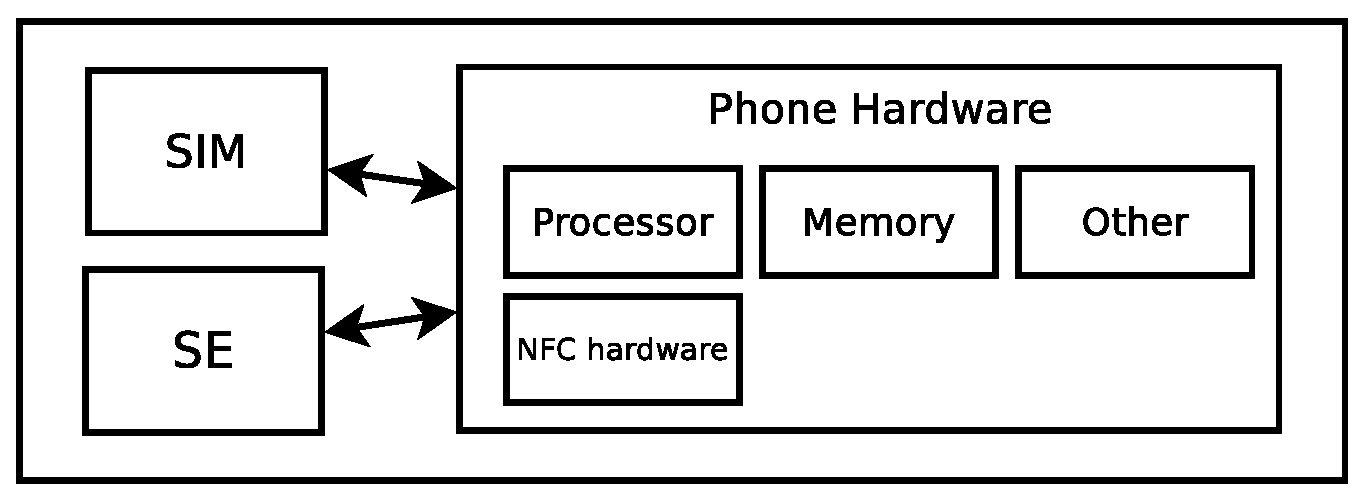
\includegraphics[width=0.9\textwidth]{images/phone_with_SE_nokia}
\caption[Nokia phone with SE]
{
A separate secure element
}
\label{fig:integrated_se}
\end{figure}


%security problems for this architecture:

%\subsubsection{Modular Secure Element}
Another option is an external SD-card which houses all the hardware needed to enable NFC and also the secure element, see figure \ref{fig:modular_se}.
%( http://www.nearfieldcommunicationsworld.com/2009/01/12/3485/tyfone-puts-nfc-into-microsd-cards/)
In this configuration a third party can issue an SD card to its customers which houses a secret key hidden from the user.

\begin{figure}
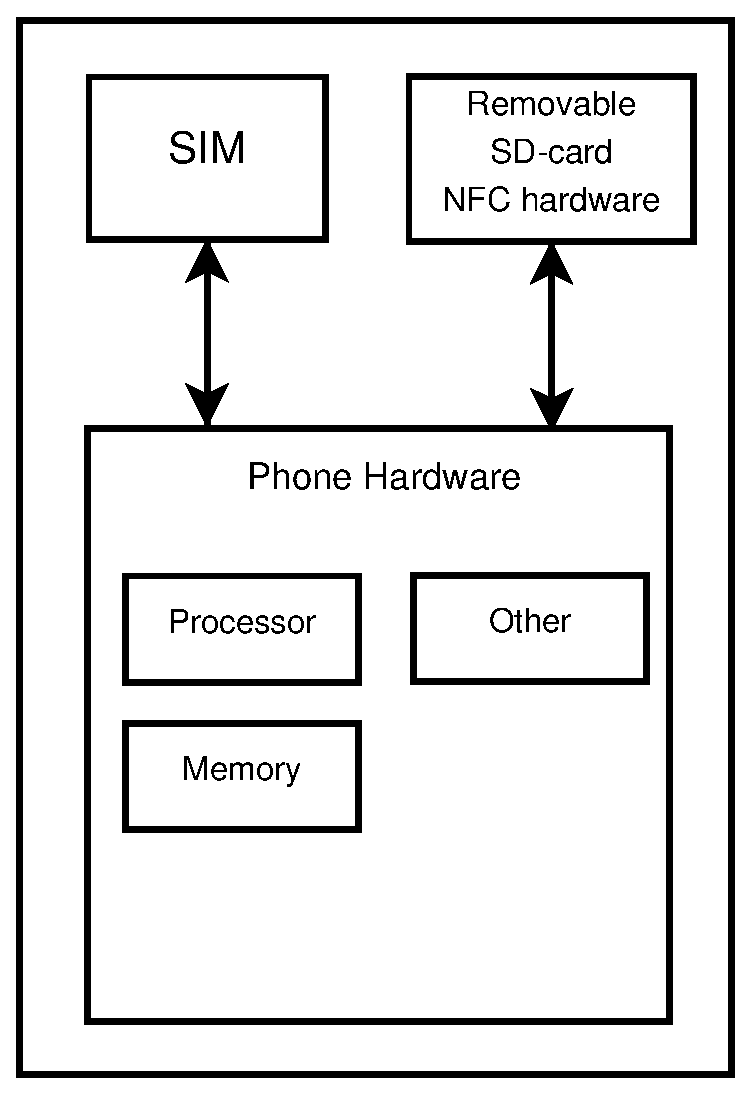
\includegraphics[width=0.9\textwidth]{images/SD_NFC}
\caption[SE in SD package]
{
An secure element in SD package
}
\label{fig:modular_se}
\end{figure}

%security problems for this architecture: SD card might get stolen and used by somebody else.
%\subsubsection{Multiple SIM cards}
Related to the above architecture is the one depicted in figure \ref{fig:multi_sim}.
Here the architecture consist of a phone with multiple SIM cards and the usual hardware.
In this case a telecom provider will own one SIM card and third-party service provider will own the other.
This way there no problem with splitting the resources of one SIM card and the trust issue between different companies.
\begin{figure}
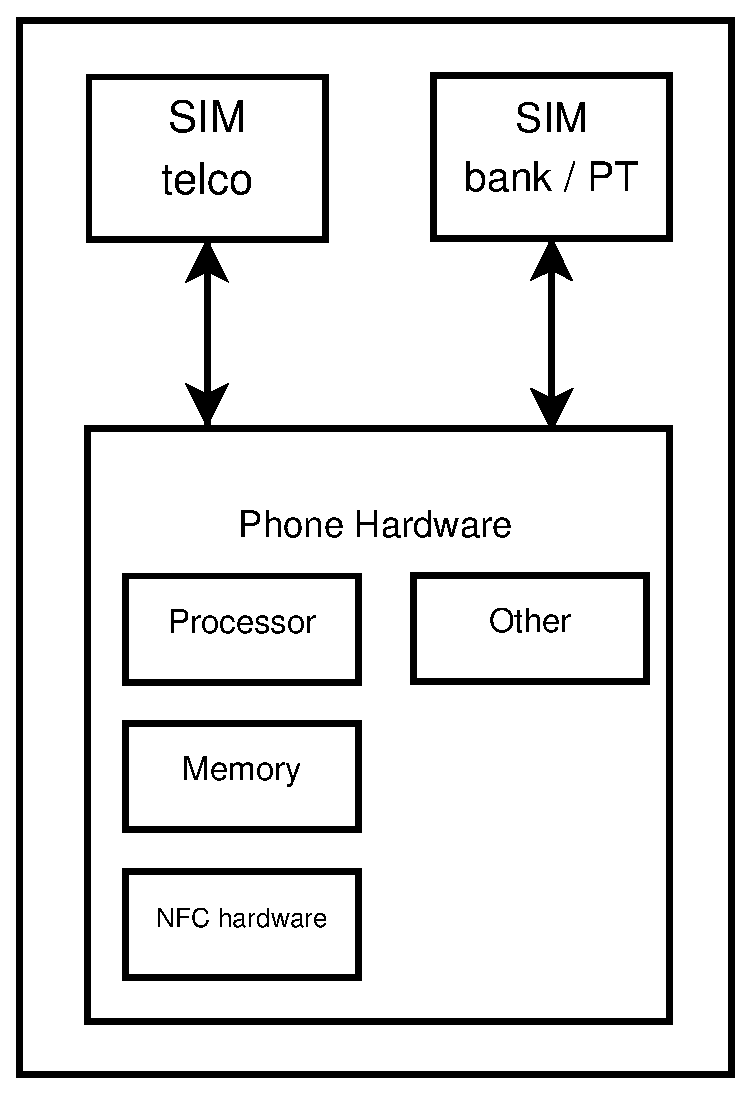
\includegraphics[width=0.9\textwidth]{images/meerdere_sims}
\caption[Multiple SIM cards]
{
Multiple SIM cards for different applications
}
\label{fig:multi_sim}
\end{figure}

%\subsubsection{Trusted SIM card}
Of course the option of splitting the resources is also possible, if different companies can find an agreement to share the same SIM card.
This is possible, because smartcards in general are becoming more powerful.
This makes two different architectures possible.
The first one, as pictured in figure \ref{fig:sim_se}, uses the SIM card as secure element.
A phone will have the usual hardware, hardware making NFC possible and SIM card with applications from the telecom provider and applications from a company chosen by the user, e.g. a bank for payment and a public transport company. 
The second option resembles a combination of the first one and the one with the SD card architecture.
Here a SIM card has all the hardware needed to make NFC possible and it also acts as a secure element (see figure \ref{fig:integrated_se}).
Like the first option, the resources of the SIM card will be split among the involved parties.
\begin{figure}
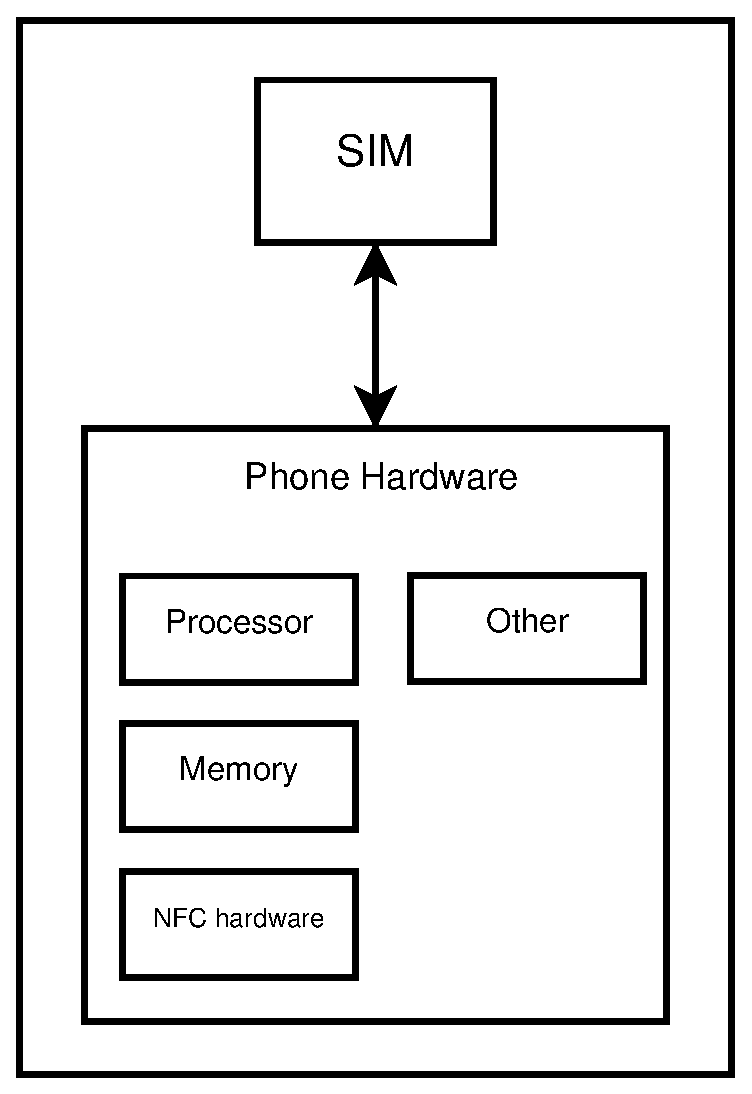
\includegraphics[width=0.9\textwidth]{images/SIM_is_SE}
\caption[Trusted SIM cards]
{
Trusted SIM card running multiple applications
}
\label{fig:sim_se}
\end{figure}

%hier moet nog een bron voor gevonden worden
%security problems for this architecture: SIM card might get stolen and used by somebody else
%hier moet nog een bron voor gevonden worden
%security problems for this architecture: SIM card might get stolen and used by somebody else


\subsection{Adoption of NFC}
In \cite{1497411} the authors investigate the possibility of running trusted code in mobile devices and concluded that while such a system is technically feasible, its widespread adoption is hampered by the certification process payment card companies impose on their payment products.
Payment card companies' current standards dictate that their cards may not be modified after production, which poses a problem as this is exactly what makes NFC an enticing alternative to conventional bank cards.

This poses a problem for the implemention of NFC in general.
As seen in (figure xx, still to add) the "demand" for NFC is a circular dependency.
If the customer doesn't demand NFC from an issuer (bank, PT), the issuer won't request a TSM to create application, so nothing will be putt on a UICC by the MNO and the customer gets nothing.
If one of the parties in this figure, refuses to cooperate, NFC will not launch.
What we see now (artikel tweakers en global platform) is that issuers and MNO are working together to make NFC available for customers.
The next thing to happen is that mobile phones will get NFC hardware and an implementation of a secure element.
With Nokia's 6131 NFC phone a first step was made for developers.
But now also Google has announced that they will introduce a NFC phone and some rumours suggest that also Apple is developing a new Iphone with NFC, see \cite{nu_artikel}.
If customers like NFC because of the possibilities it will take off and demands for other applications will be made. 

\textbf{TODO} A good reference for cyclic dependency of stakeholders can be found in the GlobalPlatform technical report.


% TODO hoort bij Wireless communication, terwijl 3.2 (Secure Elements) heel ergens anders over gaat
%\subsection{Standardization}
%NFC has been described by NFCIP-1 (Near Field Communication Interface Protocol 1) first on ISO18092, ECMA340 and ETSI %TS102 and also NFCIP-2 defined in ISO 21481, ECMA352 and ETSI TS102 312.
%With NFCIP-2, NFC became compliant with the RFID standards of ISO14443 and ISO15693.


% diagram van NFC communicatie

%TODO RFiD card vs NFC - verschil vd terminal
%                      - live GSM verbinding met de bank
%TODO Online vs Offline
%                      - privacy gevoeligheid

%\section{Wireless communication}
%The distance at which the NFC communication takes place is 10 cm, operates at the 13.56 MHz frequency and it has a transfer speed of 106, 216, 424 kbit/s.
%promising secure element alternatives for NFC technology. */


\subsection{Advantages and Limitations}
\textbf{TODO}

% Toetsenbord en display feature (semi-trusted terminal, moeilijker te tamperen)

% Voorbeeld telefoon met gewone sim en NFC SD card adapter
% Bankier kan heir apps op installeren

% Voorbeeld telefoon met meerdere sims

% Vorobeeld SIM en losse SE, met trusted code

% Voorbeeld SIM van KPN, met apps van de bank

%TODO Uitzoeken:
% Rabomobiel - SIM vd rabobank



%\chapter{Known Vulnerabilities}
%\label{chap:known_vulnerabilities}
\section{Security research}

While consumers might see NFC applications as a gadget that will make their lives easier, this development towards contactless payment systems has raised questions from security researchers.
%TODO Summarize and reference some security research done on RFID.

Because NFC will be used in payment and access control, it should be assumed that attackers will try to exploit this technology. Research has been done on the security of NFC and the results show that attacks are possible, which will be discussed below.

Because NFC will be used in payment and access control, it should be assumed that attackers will try to exploit this technology for their own gain. 
%Research has been done on the security of NFC in several areas, among which:

% TODO Referenties toevoegen
%\begin{itemize}
%\item Creating secure off-line payment applications \cite{1592613}
%\item Trusted computing using mobile applications which are managed remotely
%\item Network attacks against \textit{Wireless Personal Area} (WPAN) \textit{Networks} (e.g \textit{Denial of Service}, \textit{Snooping}, \textit{Man-in-the-middle}, etc.) \footnote{Even though NFC isn't strictly a WPAN system as it only allows for 2 communicating parties, this paper also covers network attacks against NFC.}  \cite{1506342}
%\item Intrusion detection mechanisms for WPANs \cite{1361512}
%\item Mitigations agains privacy issues related to wireless payment systems \cite{1527027}
%\end{itemize}

\subsection{Relay attacks}
% TODO
% Maar de NFC telefoon heeft toetsenbord (om actieve approval vd eigenaar te vragen (en te zeggen hoeveel er betaald gaat worden)
RFID, a technology that NFC is compatible with, is prone to relay attacks. A relay attack is a combination of a man-in-the-middle and relay attack. The goal is that the attacker will gain something, but victim will lose something, e.g. the attackers will get an item from a shop, but the victim is the one who is paying. 
To achieve this, the attacker will need a device that fakes a NFC phone or plastic NFC card (ghost) and a device that fakes a reader (leech). The ghost will be used to communicate with a genuine reader and the leech will communicate with a genuine card. The attacker must trick the user into making a legitimate purchase, and have the devices set up in such a way that they operate on much larger distance then the normal operational distance of 10 cm, because then the attack will go unnoticed. \cite{1128470}
With this attack it will also be possible to gain access to the public transport. The check-in gate will communicate with the ghost, which will pass it on to the leech, which will pass it on victim and vice versa. The check-in gate will "think" it is communicating with the victim, but because the attacker is closer to the gate then the victim, he will gain access first and the victim will pay.

\subsection{Countermeasures relay attacks}
There are three possible countermeasures, a Fareday-cage, activation by the user or Two-Factor authentication. A Fareday-cage will block all the wireless communication, so an attacker can make contact with the device. This is not a feasible countermeasure for a mobile phone, because it will not have any connectivity.
With activation of the user, the user will have to switch on NFC on the device, to be able to e.g. make a payment or use public transport. It will not be possible for an attacker to use the phone at any time. This will slighty decrease the user friendliness, because the user will have to switch NFC on and off when it will be used.
With Two-Factor authentication, the user will be asked to present something, e.g. a password, pincode or token. NFC will be turned on all the time, but only when it will be used, the user will type the pincode and a connection is made. The attacker will actually notify the user, that a connection will be made. If the user is aware that the NFC connection is not necessary (because he is not near a payment terminal) and declines or does not type the pincode, the attack is avoided. This countermeassure will also decrease the user friendliness. \cite{1128470}

Overall this attack will not be feasible, because the attacker has to be in relative close range, which will look suspicious. It will also be difficult to maintain an active connection with the terminal and the victim.


%plaatje relay attack

% 2 verschillende scenario's relay attack
% I - stiekem met iemand z'n kaart praten
% II - een frauduleus/gemhackte terminal neerzetten waar iemand - willens en wetens - z'n kaart tegenaan houdt.

\subsection{Malware distribution vectors}
One way to distribute malware is to use the smart poster.
It has proven to be possible to mislead a user to visit a malicious website through a modified NFC-tag.
By using space, tab and new line characters in the data transmitted from the RFID-tag, the attacker is could modify the title of the message so that it looks normal (with a title and URL) to the user.
The actual URL part of message is not shown to user, but it is still executed.
The user is unaware, that he or she is directed to a malicious website, from where a number of further attacks are possible.
In the same way it is possible to let the user call or send a text message to a different number, e.g. an 0900-number.

It is also possible to hide and spread a worm in this manner.
Therefore, the phone of the user has to be infected with the worm. When the phone reads a tag, it will try to change it, like described above.
The next user will be pointed to a website where he will be tricked into downloading and installing a copy of the worm.

A denial of service attack is also possible, with the goal to let users stop using the service. By using a tag that sends out malformed messages, taped on top of the original tag, the phone of the user will crash when he attempts to read the tag. \cite{mulliner2009vulnerability,rieback2006your} 

\subsection{Countermeasures malware distribution vectors}
This vector is similar to other networking attacks
The best defense against these kinds of attacks is user vigilance in spotting malicious. 

\subsection{Differential Power Analysis Attack}

A Differential Power Analysis (DPA) attack is a form of side channel attack. A side channel attack is based on information that can be collected by analysing the physical implementation of a cryptographical system (cryptosystem) e.g. power usage, electromagnetic leakage or timing. It is possible to prevent this from happening, by implementing extra shielding, filtering inputs and outputs. This is a problem for devices where the cryptosystem has to be small, cheap and low on power usage e.g. the secure element in a mobile device.

With DPA the power consumption is measured to extract information about the workings of the cryptosystem. To measure the power consumption an analog to digital converter is used. When the cryptosystem is processing, the power usage will vary during the different operations. The information is statistically analyzed to determine the key or data, or it can give information about the key, which can help to speed up the attack or help a different attack to succeed. This technique can also be applied for electromagnetic radiation. Information can also be collected from signals generated by data travelling to and from the secure element and memory.
All these variations in ICC, wires and electromagnetic radiation can provide information to be analyzed to yield some information about the key or secret data.

One measurement of these variations might not be enough to produce the entire key, because of noise (e.g. inaccuries, outside influence) that is collected during the measurement, which will provide no information about the key. Therefore several measurements are necessary to distinguish the signal from the noise. By aligning the meassurements, an attacker can compare data on single points of interest. By averaging the collected data, the usable signal is amplified and the noise is filtered out.

Another way to collect information about the key, besides taking many different measurements, are changing some bits of the key to check if the changes might reveal some information about process. This technique can also be repeated and statiscally analyzed to get the key. Also by resetting or switching off the power during a specific operation, which can be repeated, information about the key might be collected.

\subsection{Countermeasures Differential Power Analysis}
A DPA attack is succesful if enough information can be collected to retrieve the key in the cryptosystem. By increasing the number off measurements, it will take more time to collect the information needed to retrieve the key. 
There are several ways to increase the number of measurements. For example, randomly generated noise can be added to the operations of the cryptosystem, which will make harder to filter out the signal, because more measurements are needed. Another way is to reduce the signal size, making it harder to pick up. 
If the cryptosystem is designed to self-destruct (it brakes) after a certain amount of operations and the number of measurements needed to retrieve the key is higher then amount of operations, the key can not be retrieved.

Another countermeasure to prevent information from being collected is clock skipping. Normally a cryptosystem uses an external clock for its processing, with clock skipping an internal clock is used in the cryptosystem. This will create more noise and will prevent the attacker aligning the points of interest in the collected data and making it more difficult to identify the signal. 



% ERIk open platform vs gesloten platform

%TODO Countermeasures

\section{Future work}
\label{chap:future_work}

- The application of NFC in the healthcare system is very interesting. Consequences of security problem and how it relates to health, needs to be researched. It's an upcoming technology....

- Possibly mention the cyclic dependency problem between involved parties again.

- While the possibility of secure offline payments using NFC is intruiging, the hardware is not yet powerful enough to accomodate transfers swiftly.

\label{chap:conclusions}
\section{Conclusions}

At the start of this research we had the following research question and hypothesis. 

\begin{quote}
What is the security architecture of NFC applications for mobile devices and what are some of the known and foreseen vulnerabilities?
\end{quote}

\begin{quote}
\textit{We think that most new vulnerabilities will be found in applications built on top of NFC systems, rather than in the NFC architecture itself.
We envision vendors might try to apply existing business rules to this new system, even if their understanding of it is oversimplified.}
\end{quote}

During our research we looked at several possible applications for NFC currently being developed and tested.
The most likely applications to initially make use of NFC appear to be payment and public transport.
In these two sectors it is likely that NFC will become available for consumers, because pilots have been started in these sectors and a lot of research has been done into making these applications feasible.
Because of the current stage of affairs in the development of NFC applications, we were unable to test this hypothesis thoroughly.

Making use of the UICC to function as a Secure Element as proposed by GlobalPlatform is hampered by the reluctance of Mobile Network Operators to share the resource with other parties.
The network attacks summarized in this paper are practical attacks against SEs that behave similar to RFID tags, and work regardless of the internal architecture employed by the handset for accessing its SE.

%The concept of an electronic currency as explored by \textit{mFerio} seems very promising
%It's possible for the mobile handset to become a high- target
We find it likely that the development of malware for smartphones will be boosted when the deployment of NFC payment applications becomes widespread.
Smartphone devices, which often already play a central role in their user's lives, will actually become directly financially valuable for criminal interests.

%Chicken egg problem + verschillende nadelen per architectuur + niet duidelijk welke architectuur het wordt.

%The known vulnerabilities are applicable to all of the SE integration architectures mentioned above.
%It does not matter that the secure element is owned by one party or shared by multiple parties.
%It also does not matter how the secure element is implemented in the architecture of the mobile device.
%The attacks mentioned in chapter 4 all apply to the different architectures mentioned in chapter 3. 

%As mentioned in paragraph 4.5 differential power analysis is a problem for devices where the secure element has to be small, cheap and have low powerusage.


\newpage

%\begin{figure}
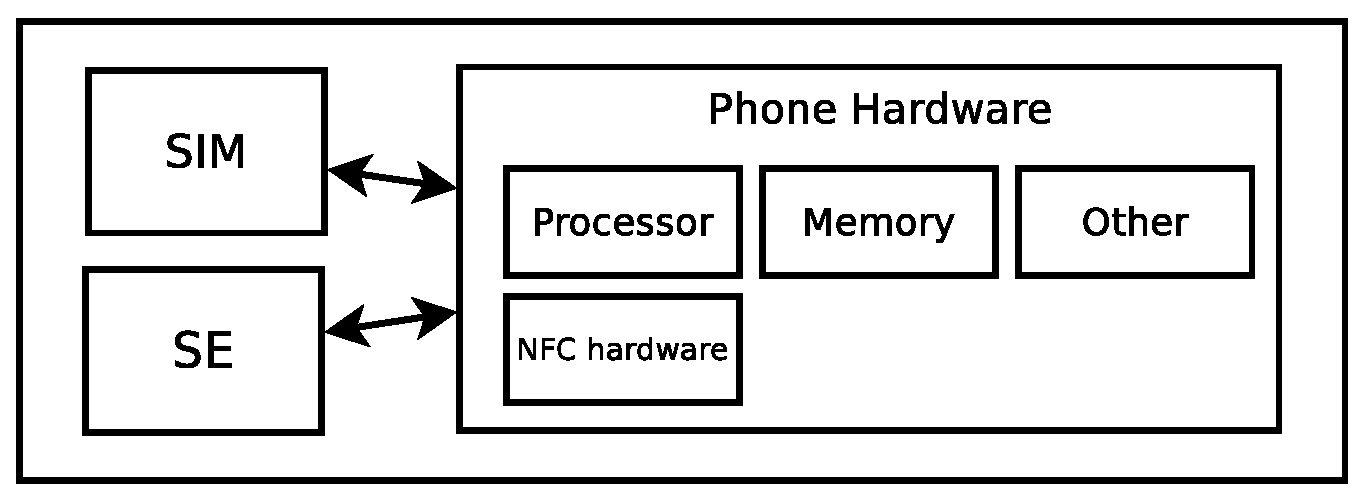
\includegraphics[width=0.5\textwidth]{images/phone_with_SE_nokia}
\caption[Nokia phone with SE]
{
A separate secure element
}
\label{fig:integrated_se}
\end{figure}

\begin{figure}
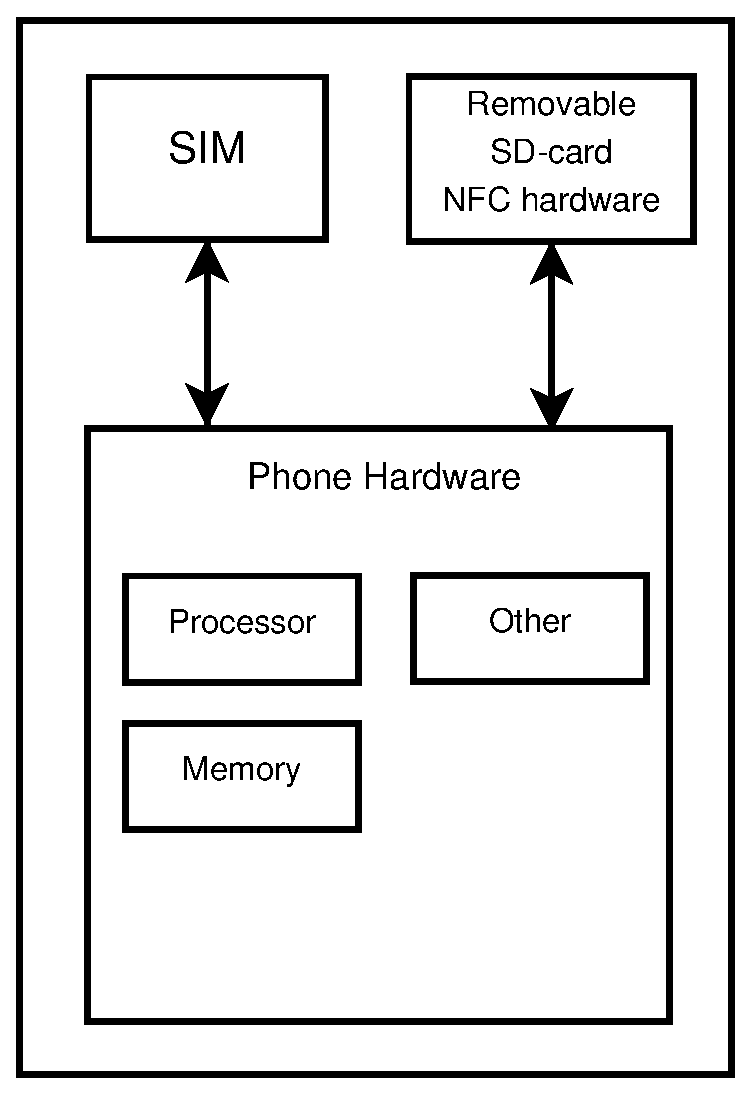
\includegraphics[width=0.5\textwidth]{images/SD_NFC}
\caption[SE in SD package]
{
An secure element in SD package
}
\label{fig:modular_se}
\end{figure}

\begin{figure}
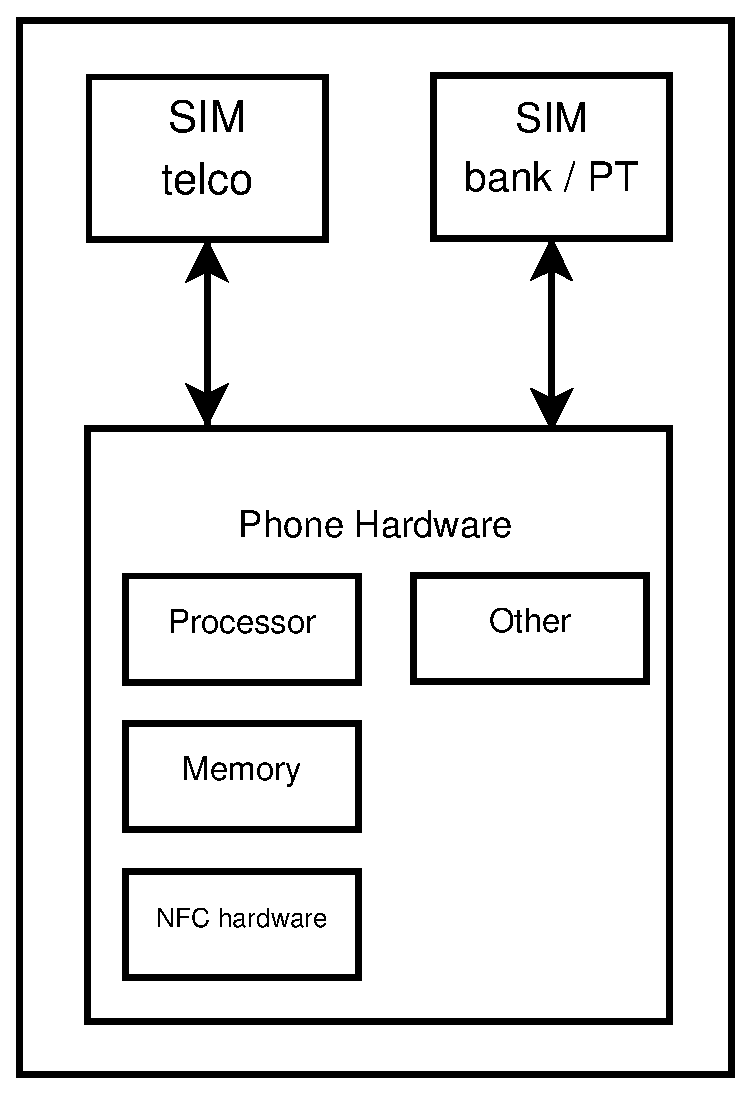
\includegraphics[width=0.5\textwidth]{images/meerdere_sims}
\caption[Multiple SIM cards]
{
Multiple SIM cards for different applications
}
\label{fig:multi_sim}
\end{figure}

\begin{figure}
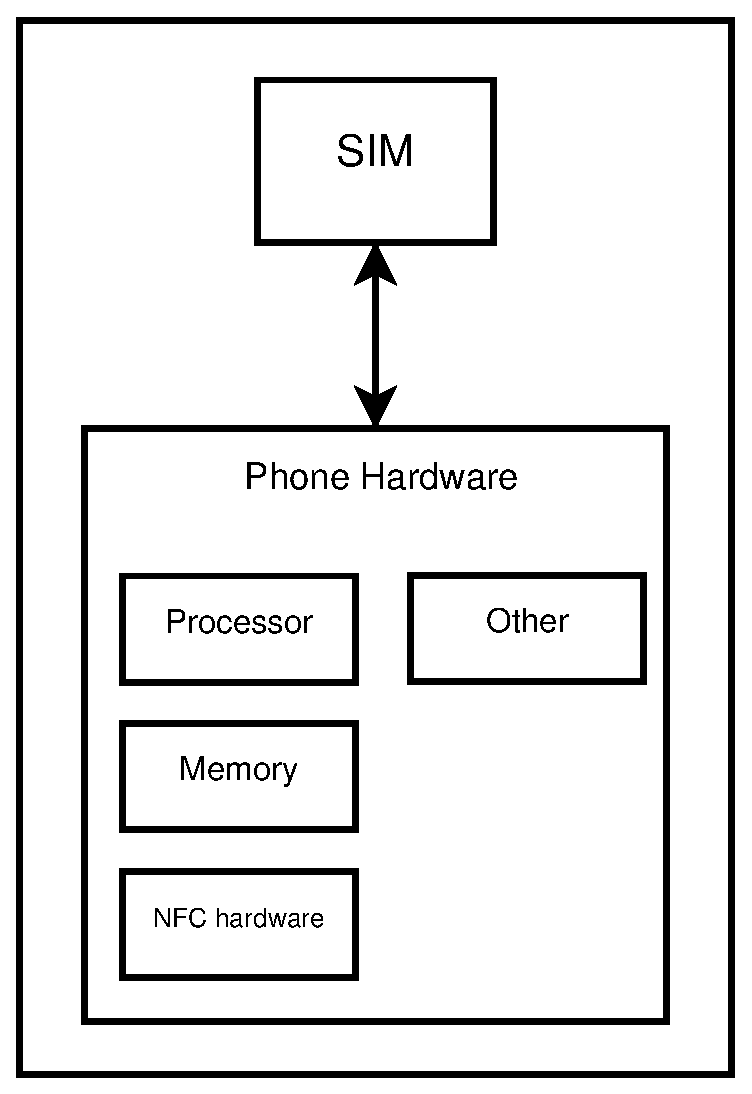
\includegraphics[width=0.5\textwidth]{images/SIM_is_SE}
\caption[Trusted SIM cards]
{
Trusted SIM card running multiple applications
}
\label{fig:sim_se}
\end{figure}




%\cleardoublepage

%\newpage

\bibliographystyle{alpha}
\bibliography{rdr1}
%\printglossaries

\end{document}

